%%% Meetup PostgreSQL Paris

\documentclass{beamer}

\usepackage[utf8]{inputenc}

\usepackage{beamerthemesplit}
\usetheme{Boadilla}
\setbeamertemplate{itemize items}{\checkmark}
%\setbeamertemplate{itemize items}[circle]
\beamertemplatetransparentcovered

\usepackage{multicol}

\title{PostgreSQL Meetup}
\subtitle{PARIS}
\author{Dimitri Fontaine \texttt{dimitri@2ndQuadrant.fr}}
\date{April 16, 2014}
\logo{
\includegraphics[height=0.4cm]{2ndQuadrant-cross.png}}

\begin{document}

\frame{\titlepage}

\begin{frame}[fragile]
  \frametitle{PostgreSQL Meetup}

  \center{Les clubs de rencontres... d'utilisateurs}
  \vfill

\begin{columns}
\column{.4\textwidth}

  \begin{itemize}
  \item San Francisco
  \item Portland (PDX)
  \item New York
  \item Et pourquoi pas Paris ?
  \end{itemize}

\column{.6\textwidth}
\begin{center}
  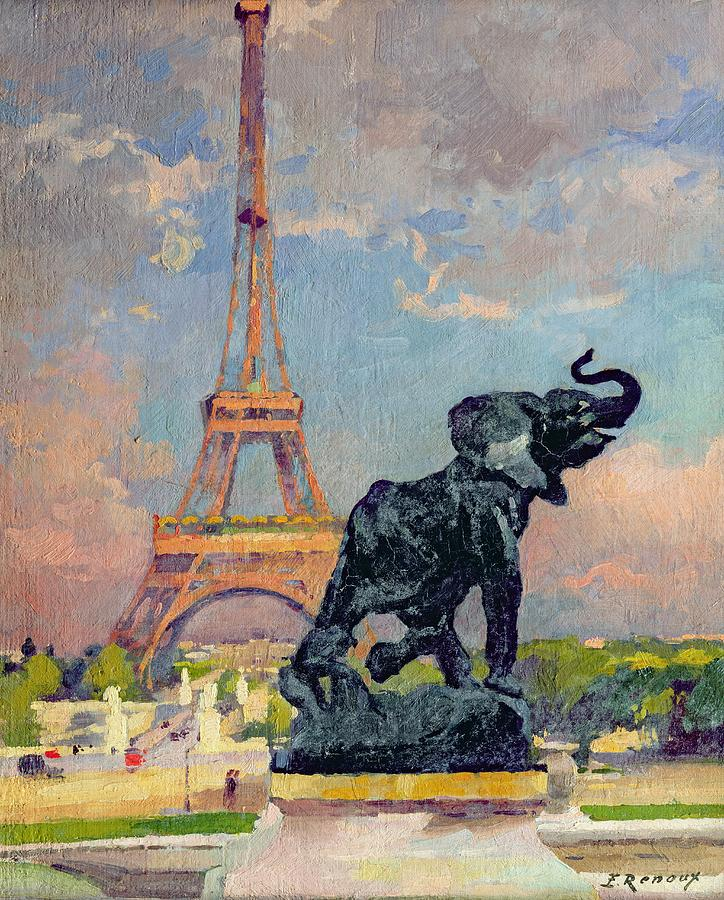
\includegraphics[height=15em]{the-eiffel-tower-and-the-elephant-by-fremiet-jules-ernest-renoux.jpg}
\end{center}
\end{columns}
\end{frame}

\begin{frame}[fragile]
  \frametitle{Déroulement d'un Meetup}

  \center{Partage et échange dans un cadre professionel}
  \vfill

\begin{columns}
\column{.7\textwidth}

\begin{itemize}
\item \textit{Partage} de connaissances
\item \textit{Échange} de nouvelles idées
\item Mini-Conférence : une seule présentation
\item \textit{Lightning Talks}
\item Buffet (pizza et bières)
\end{itemize}

\column{.3\textwidth}
\begin{center}
  
\includegraphics[height=6em]{conferences.jpg}
\end{center}
\end{columns}
\end{frame}

\begin{frame}[fragile]
  \frametitle{Financement par des sponsors}

  \center{Il parait que les professionnels ils ont du budget}
  \vfill

\begin{itemize}
\item Mise à disposition d'un lieu, ce soir, \textbf{eNovance}
\item Mise à disposition du buffet, ce soir, \textbf{Hegoa}
\end{itemize}
\end{frame}

\begin{frame}[fragile]
  \frametitle{Hegoa}

  \begin{center}
    
\includegraphics[height=1.1in]{hegoa.png}
  \end{center}
\end{frame}

\frame{
  \frametitle{Aujourd'hui}

  \begin{center}
    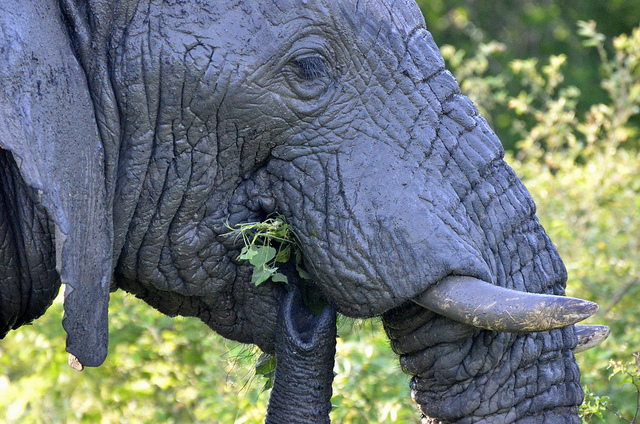
\includegraphics[height=9em]{postgresql-mongodb.jpg}
  \end{center}

\begin{itemize}
\item PostgreSQL et OpenStack, \textbf{Julien Danjou}
\item PostgreSQL et la sécurité intérieure, \textbf{Vincent Laborie}
\item Un Tsung vaut mieux que deux "croisons les doigts" !
  \linebreak \textbf{Rodolphe Quiédeville}
\end{itemize}}

}

\end{document}
